\chapter{Respostas Qualitativas dos Participantes}
\label{appendix:respostas-qualitativas}

% Usar o graphicspath para buscar figuras no subdiretório figuras
\graphicspath{\currfiledir/figuras/}

Este apêndice apresenta as respostas qualitativas completas dos participantes
coletadas através do questionário Google Forms. As perguntas abertas permitiram
aos participantes expressar suas opiniões detalhadas sobre aspectos específicos
da ferramenta, complementando a análise quantitativa apresentada na Seção
\ref{subsec:analise-qual}.

\begin{figure}[H]
\centering
\includegraphics[
    page=6,
    trim={1cm 6cm 1cm 1cm},
    clip=true,
    width=0.9\textwidth
]{../4-valida/forms.pdf}
\caption{(Parte 1) "O que mais gostou?" - Comentários dos participantes sobre os
aspectos mais valorizados da ferramenta.}
\label{fig:respostas-qual-1-parte1}
\end{figure}

\clearpage

\begin{figure}[H]
\centering
\includegraphics[
    page=6,
    trim={1cm 1cm 1cm 22cm},
    clip=true,
    width=0.9\textwidth
]{../4-valida/forms.pdf}
\caption{(Parte 2) "O que mais gostou?" - Comentários dos participantes sobre os
aspectos mais valorizados da ferramenta.}
\label{fig:respostas-qual-1-parte2}
\end{figure}

\begin{figure}[H]
\centering
\includegraphics[
    page=7,
    trim={1cm 6cm 1cm 1cm},
    clip=true,
    width=0.9\textwidth
]{../4-valida/forms.pdf}
\caption{(Parte 1) "O que poderia melhorar?" - Sugestões de melhorias e
limitações identificadas pelos participantes.}
\label{fig:respostas-qual-2-parte1}
\end{figure}

\clearpage

\begin{figure}[H]
\centering
\includegraphics[
    page=7,
    trim={1cm 1cm 1cm 22cm},
    clip=true,
    width=0.9\textwidth
]{../4-valida/forms.pdf}
\caption{(Parte 2) "O que poderia melhorar?" - Sugestões de melhorias e
limitações identificadas pelos participantes.}
\label{fig:respostas-qual-2-parte2}
\end{figure}

\begin{figure}[H]
\centering
\includegraphics[
    page=8,
    trim={1cm 15cm 1cm 1cm},
    clip=true,
    width=0.9\textwidth
]{../4-valida/forms.pdf}
\caption{(Parte 3) "O que poderia melhorar?" - Sugestões de melhorias e
limitações identificadas pelos participantes.}
\label{fig:respostas-qual-2-parte3}
\end{figure}

Estas respostas qualitativas forneceram a base para a análise temática
apresentada na Seção \ref{subsec:analise-qual}, permitindo identificar padrões
recorrentes nos comentários dos participantes e direcionamentos específicos para
melhorias futuras da ferramenta.
